\section{Overview}
\label{sec:overview}

\begin{figure}
  \centering 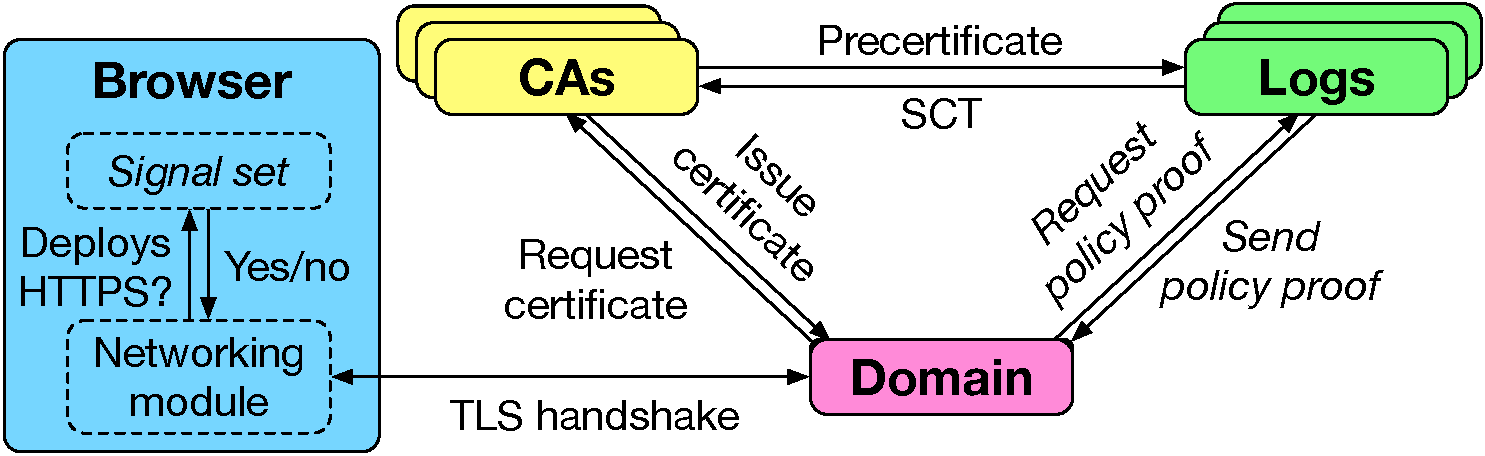
\includegraphics[width=\linewidth]{fig/overview} \caption{Overview
    of \ac{name} architecture (log auditors and monitors not shown). The browser
    is part of the client. Dotted lines denote browser components, and italic
    text denotes new components or actions in \ac{name}.}
  \label{fig:overview}
\end{figure}

In this section, we present a high-level overview of \ac{name}. We first present
one of our central insights and then describe the \ac{name} architecture. We
then provide an intuitive explanation for the policy and signaling mechanisms.

To move towards \iac{pki} with increased resilience to the compromise of trusted
parties (i.e., \acp{ca}), we need to prevent \iac{ca} that misissues a
certificate for a domain from exposing that domain to \iac{mitm} attack. We
observe that signatures from multiple independent \acp{ca} on a single public
key can spur greater trust in the key, and therefore we design \ac{name} around
the idea that domains should be able to obtain and communicate the presence of
multiple certificates for a single public key. We can then protect domains from
\ac{mitm} attacks by simply communicating to the client the number of
certificates to expect. This approach results in simple policies that require
domain involvement only in rare cases of deliberate misissuance, and allow
security-conscious domains to ``ratchet up'' their security to their desired
level.

\ac{name} leverages \ac{ct}'s infrastructure in its policy mechanism, and
therefore the two systems have similar architectures, as shown in
\autoref{fig:overview}. \steve{TODO: add Censys data and an external service or
browser vendor to the overview figure} \ac{name} assumes a full deployment of
\ac{ct}, that is, all certificates must be logged for clients to accept them as
valid. \steve{Beginning in October 2017, Chrome will begin enforcing this
  requirement for all \ac{https} sites, so this assumption is a reasonable one.}
  For the purposes of obtaining \acp{sct}, the logging process works just as it
  does in \ac{ct}. Also as with \ac{ct}, public logs are kept accountable by
  auditors and monitors, and an external party (Google in the case of \ac{ct})
  maintains a list of known trusted logs.

In \ac{name}, however, logs maintain an additional database of certificate
policies alongside their database of certificates. The logging process also
triggers changes in this policy database. Domains periodically request the proof
for their latest policy from the logs and provide both their policy and proof to
clients during the \ac{tls} handshake. We further describe the details of our
policy mechanism in \autoref{sec:policy}.

Client browsers locally maintain a \emph{signal set}, which indicate whether or
not a given domain has deployed \ac{https}. The browser queries the signal set
before initiating an HTTP or \ac{https} connection to a site 
in order to determine
\begin{inparaenum}
\item whether or not to establish \iac{https} connection, and
\item if so, how many certificates to expect.
\end{inparaenum}
If the signal set indicates that the domain has deployed \ac{https} but the
server does not provide a certificate, the browser aborts the connection,
assuming that an adversary is attempting to mount \iac{tls} stripping attack.

The signal set is created by using data from the \ac{ct} logs. This data is used
to construct a list of all DNS names for which a \ac{tls} certificate has been
observed (either as the main subject or as a subject alternative name). This
list is then represented using \iac{dafsa} that recognizes the DNS names of
sites that deploy \ac{https}. By using compression techniques, we compact this
\ac{dafsa} into a representation that requires little storage. Such a compact
representation allows us to store the \ac{dafsa} in memory, offering performant
lookups. We further describe the details of our signal set design in
\autoref{sec:signaling}.

%In particular, in \ac{name} we make use of a \emph{signal set},
%stored locally by client browsers. Browsers query for the presence or absence of
%a given domain name in the signal set to determine whether that domain has
%deployed \acs{https}. Because Censys~\cite{durumeric2015search} currently
%reports that close to 70 million known domains deploy \ac{https} and Verisign
%reports almost 330 million domain names overall~\cite{dnib-14-1}, we design our
%signal set to be scalable to hundreds of millions \steve{or billions, hopefully}
%of names, while taking up minimal space on client devices and supporting
%efficient membership queries. While \ac{ct} leverages public append-only logs to
%ensure that any \ac{ca} misbehavior for domains that have deployed \ac{https}
%must be made publicly visible before \iac{mitm} attack, the use of a signal set
%prevents an attack that can be made even with full \ac{ct} deployment, in which
%an adversary tries to fraudulently convince a client that a domain has not
%deployed \ac{https}. In \autoref{sec:signaling}, we provide a detailed
%look at our signal set design.

%\ac{name} further adds misbehavior prevention to the misbehavior detection
%capabilities of \ac{ct} through the use of \steve{policies for domains
  %maintained at public logs}. Specifically, public logs in \ac{name} maintain
  %policies for each domain that encode \steve{\acp{ca} authorized to issue
  %certificates for a domain or the number of independent certificate chains a
%domain must present to the client}. In contrast to other extensions of \ac{ct}
%that use log-based certificate policies such as
%PoliCert~\cite{szalachowski2014policert}, these policies do not need to be
%directly specified by the domain. \steve{I suppose this leaves out authorized
  %\ac{ca} specification unless we are willing to admit errors using a heuristic
%approach.} In \autoref{sec:policy}, we provide a detailed look at our policy
%mechanism.

%For comparison, we first present a
%purely DNS-based approach.

%\subsection{DNS-Based Policy}

%DANE~\cite{rfc6698} allows domains to specify policies (in the form of TLSA
%resource records in DNS) governing their public key certificates. Specifically,
%domains can specify
%\begin{compactenum}
%\item a CA certificate or public key that must appear in that domain's
  %certificate chain,
%\item a leaf certificate or public key that must be sent by the domain to the
  %client during the TLS handshake,
%\item a certificate or public key that must be used as the trust anchor of a
  %certificate chain (effectively allowing the domain to declare its own root
  %CA), or
%\item a leaf certificate or public key that must be sent by the domain to the
  %client, but does not need to be chained to a client-accepted root CA (i.e.,
  %the domain effectively sends a self-signed certificate).
%\end{compactenum}
%DANE thus provides domains with a great deal of flexibility: domains can prevent
%certificates issued by other misbehaving CAs or those certifying any other key
%from being accepted by clients, and domains can even eschew the CA hierarchy
%altogether by specifying their own trust roots or certificates.

%If a domain continues to obtain certificates from CAs, it can make use of the
%Certificate Authority Authorization (CAA) resource record~\cite{rfc6844}, which
%allows the domain to specify which CAs are authorized to issue certificates for
%the domain. In contrast to its counterpart in DANE, however, a CAA resource
%record is checked by CAs when the certificate is issued. Before issuing a
%certificate for a domain, a CA should check if a domain has a CAA resource
%record and ensure that the CA's name is present in the record. Though nothing
%stops a misbehaving CA from failing to check for a CAA resource record, the
%CA/Browser Forum has recently made this checking
%mandatory,\footnote{\url{https://cabforum.org/2017/03/08/ballot-187-make-caa-checking-mandatory/}}
%meaning that any CA that wants to continue issuing EV certificates (a capability
%granted by the CA/Browser Forum) must perform this check.

%With these systems in place, a domain can register its DNS name and obtain
%DNSSEC resource records (either creating these records itself if it manages its
%own nameserver or having its registrar manage the records). The domain can then
%create a CAA record restricting the CAs that can issue certificates for the
%domain (if obtaining CA-issued certificates), and also create a TLSA record to
%communicate this information to clients. Clients can then determine criteria for
%the domain's certificate chain upon receiving the DNS response, and use this
%information to determine whether or not to accept the presented certificate
%chain during the TLS handshake.

%A number of shortcomings exist with this approach. First, an adversary only
%needs to compromise a single private key (that of the registrar) to generate an
%unauthorized certificate that will be accepted by clients. Namely, the adversary
%can create a false TLSA record for a domain and use this to present a
%certificate (even a self-signed one) that the client would accept. However, the
%adversary cannot carry out targeted attacks this way (because DNSSEC must return
%a consistent response for all queries), and thus the attack can be detected
%(though not prevented). Moreover, this approach requires reliance on DNSSEC for
%security (deployed by a very small number of domains today).

%\subsection{Signaling Multiple Chains}

%A domain can signal that it has multiple certificate chains in one of two ways.
%The domain can signal the number of certificate chains the client should expect
%through DNS or register this number with browser vendors, who then periodically
%push a collection of these values to clients.

%To signal the number of expected certificates through DNS, the domain simply
%creates a special DNS record that indicates a value representing represents the
%minimum number of certificate chains the client should expect. Specifically, we
%allow the domain to create a DNS TXT record~\cite{rfc1035} containing a string
%of the form \texttt{domain-min-chains-N} where \texttt{N} is the number of
%certificate chains that the client should expect. Alternately, we propose a new
%DNS record called the TLSC record whose resource data consists of a single octet
%representing the number of chains.

%For security purposes, the domain should authenticate the above records with
%DNSSEC. However, the deployment rate of DNSSEC is currently quite low at around
%$0.6\%$ of the most popular sites~\cite{matsumoto2017ikp}. We thus expect that
%few domains will make use of this approach in practice; nevertheless, we allow
%this approach in addition to the one below to ensure that domains can easily
%signal the use of multiple certificate chains.

%To signal the number of expected certificates through the browser, the domain
%contacts one or more \emph{registration authorities}. At a high level, these
%registration authorities maintain an authenticated mapping of domain names to
%the minimum number of independent certificate chains that the client should
%expect. Because the set of domain names is finite (though large, at around 330M
%names in total) and the set of domains with multiple certificate chains is
%expected to be relatively small, we can leverage a set of filter cascades
%similar to that of CRLite~\cite{larisch2017crlite}. In particular, we can assume
%that the majority of domains will continue to use only a single certificate
%chain, with the number of domains using $n$ certificate chains falling sharply
%as $n$ increases. Let $U$ be the set of all domains, so $|U|$ is the number of
%all domains. Then, following the CRLite analysis, even in the absolute worst
%case (the number of domains with multiple certificate chains is $|U|/2$), a
%filter cascade would be about $0.35|U|$ bytes in size.

%\subsection{Multi-Chain Handshake}

%\begin{figure}
  %\centering
  %\begin{msc}{}
    %\setlength{\instdist}{6.0cm}
    %\setlength{\envinstdist}{1.0cm}
    %\setlength{\instwidth}{0.9cm}
    %\declinst{cli}{\scriptsize{Client}}{}
    %\declinst{dom}{\scriptsize{Domain}}{}

    %\mess{\scriptsize{ClientHello}}{cli}{dom}
    %\nextlevel
    %\mess{\scriptsize{ServerHello, Chains, ServerKeyExchange,
    %ServerHelloDone}}{dom}{cli}
    %\nextlevel
    %\mess{\scriptsize{ClientKeyExchange, ChangeCipherSpec, Finished}}{cli}{dom}
    %\nextlevel
    %\mess{\scriptsize{ChangeCipherSpec, Finished}}{dom}{cli}
  %\end{msc}
  %\caption{Message sequence diagram for the multi-certificate handshake. The
  %messages sent are identical to those for the \ac{tls} handshake except that
%multiple certificate chains can be sent in the handshake.}
  %\label{fig:handshake}
%\end{figure}

%In order for clients to process multiple certificate chains, we modify the
%standard \ac{tls} handshake as shown in \autoref{fig:handshake}. Our handshake
%differs from that of \ac{tls} only in the Chains message, which allows the
%server to send one or more certificate chains rather than a single chain.

%As in \ac{tls}, each chain must begin with the domain's certificate (i.e., the
%subject name of the certificate is the domain's DNS name), and in each chain,
%each certificate must be certified by the one following it. We add the
%requirement that the set of certificate chains must certify a common key.
%Ideally, the leaf certificate of each chain would specify the same key, but we
%do not assume that this will be possible for all domains.

%To allow domains to keep their existing \ac{tls} public keys while
%transitioning to a multi-chain ecosystem, we introduce an extension to
%\acs{x509} certificates called the \emph{Subject Alternative Key} extension.
%This extension allows a domain to specify additional key identifiers in
%\iacs{x509} certificate. Specifically, the extension consists of \iac{oid}
%assigned to the extension and a sequence of key identifiers encoded as octet
%strings. A key identifier is a unique value derived from a public key, such as
%the SHA-3 hash of the public key (other methods for generating key identifiers
%are discussed in RFC 5280~\cite{rfc5280}).

%The client then validates the set of certificate chains by verifying the
%following:
%\begin{compactitem}
%\item Each certificate
  %\begin{inparaenum}
  %\item has a valid signature,
  %\item is currently valid according to its NotBefore and NotAfter validity
    %period, and
  %\item has no critical \acs{x509} extensions that the client cannot process,
  %\end{inparaenum}
%\item With the exception of the last certificate in each chain, the signature on
  %each certificate can be verified with the public key listed in the Subject
  %Public Key field of the following certificate in the chain, or with the public
  %key of a root \acs{ca} known to the client.
%\item Each chain has a certificate that can be verified with the public key of a
  %root \ac{ca} known to the client.
%\item There exists a public key $K$ such that in each chain, the first
  %certificate of the chain contains $K$ as its Subject Public Key or as a
  %Subject Alternative Key.
%\end{compactitem}

